% Chapter Template

\chapter{Comparison} % Main chapter title
\label{Chapter5} % Change 5 to a consecutive number; for referencing this chapter elsewhere, use \ref{Chapter5}


\section{Architectural Differences}

\subsection{Framework \& Library}


\subsection{Real \& Virtual DOM}


\subsection{Templates: HTML \& JSX}


\subsection{TypeScript \& JS}


\subsection{Components}


\subsection{State Management}


\subsection{Data Binding}


\section{React Native \& IONIC}


\section{Testing}


\section{Learning Curve}


\section{Performance}


\section{Popularity}


\section{Popularity and future}


\begin{figure}[h!]
	\begin{center}
		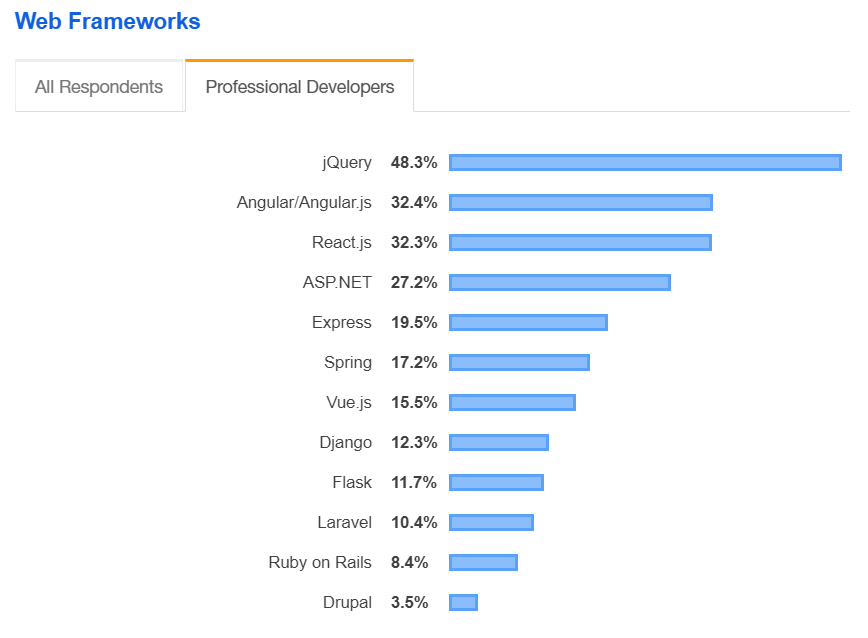
\includegraphics[scale=0.35]{images/ReactJS-VS-Angular-Survey-Stackoverflow.png}
	\end{center}
	\caption{ReactJS-VS-Angular-Survey-Stackoverflow}
\end{figure}

My search in google trends

\begin{figure}%
	\centering
	\subfloat[Trends during 16/06/2015-2019]{{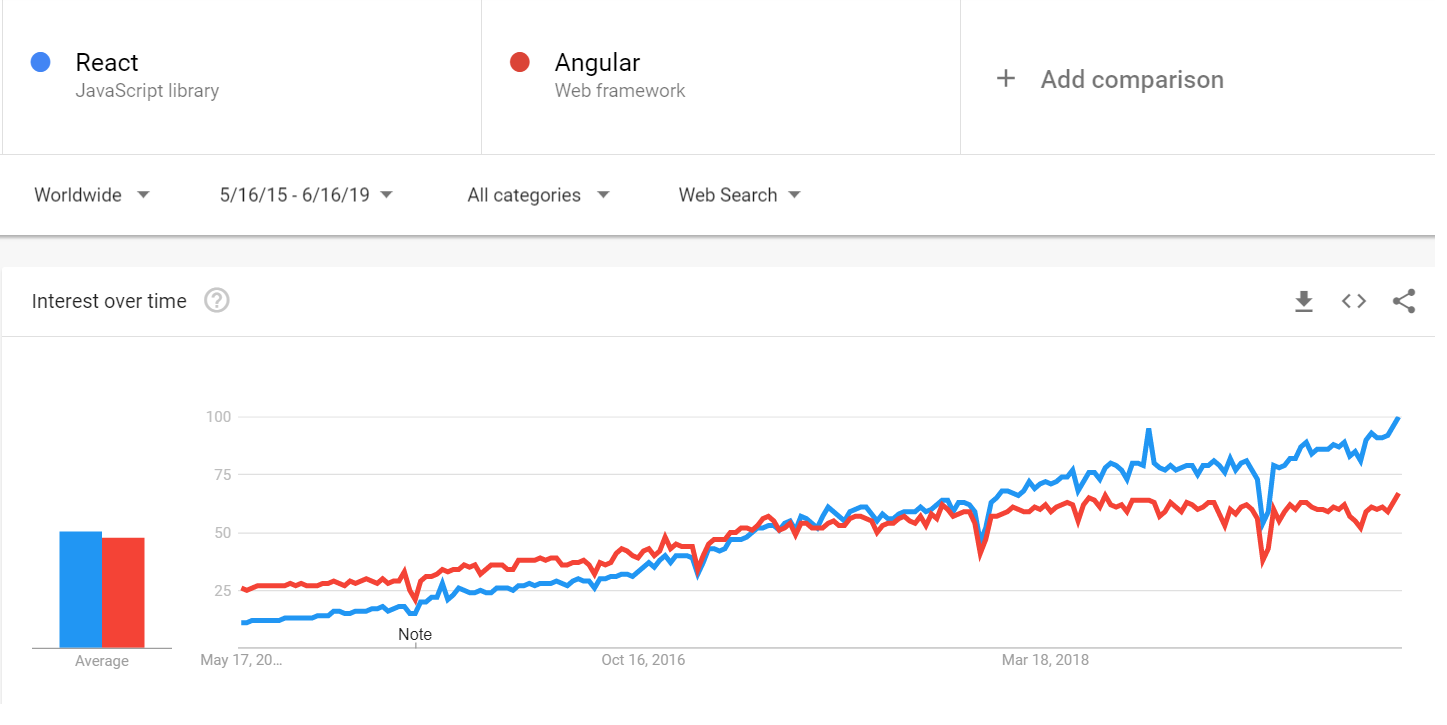
\includegraphics[scale=0.16]{images/ReactJS-VS-Angular-Google-Trends.png} }}%
	\qquad
	\subfloat[Countries' preferences]{{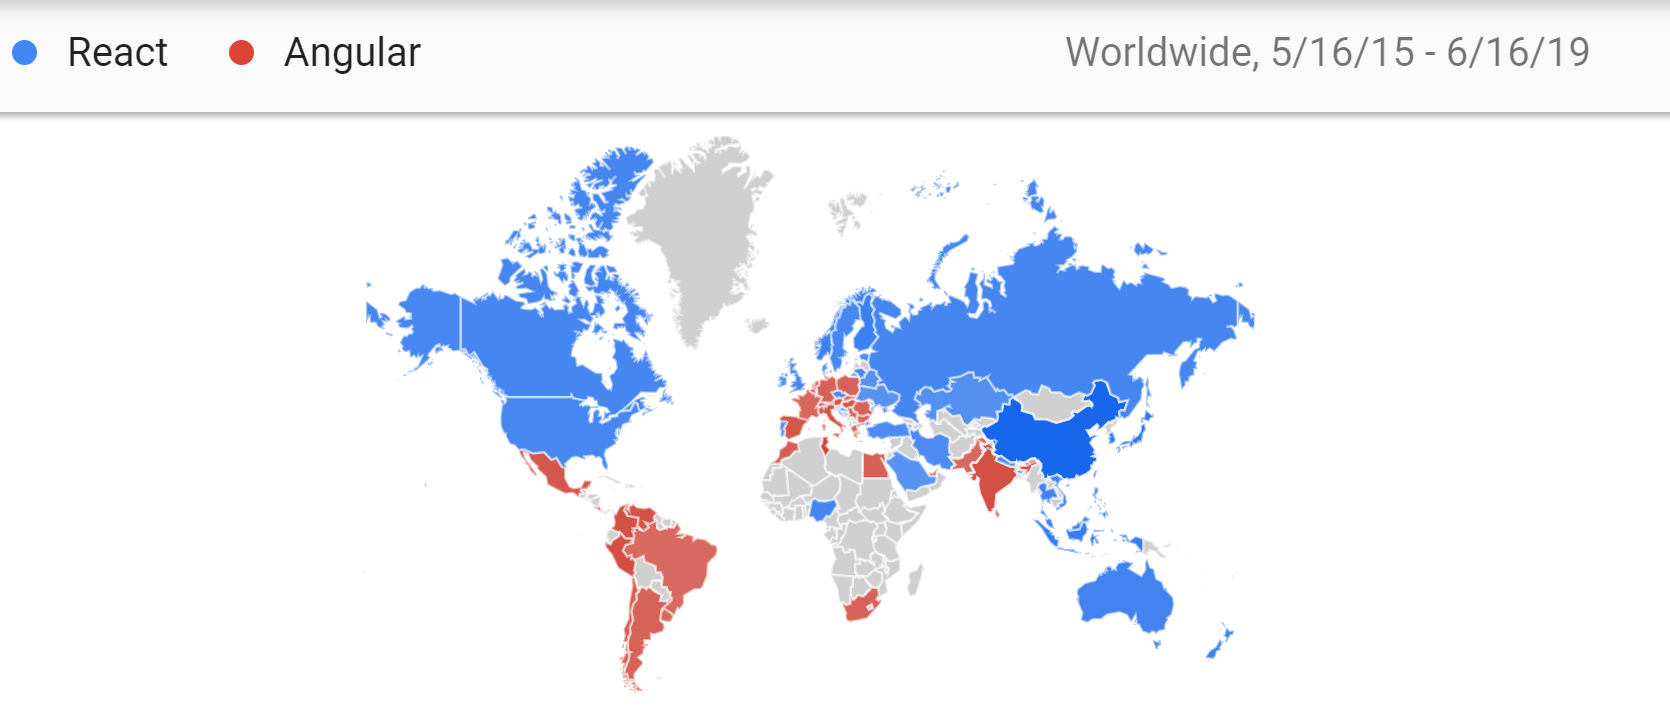
\includegraphics[scale=0.16]{images/ReactJS-VS-Angular-Google-Trends-Map.png}}}%
	\caption{ReactJS VS Angular in Google Trends}%
	\label{fig:example}%
\end{figure}

My search in npm trends (https://www.npmtrends.com/react-vs-@angular/cli)

\begin{figure}[h!]
	\begin{center}
		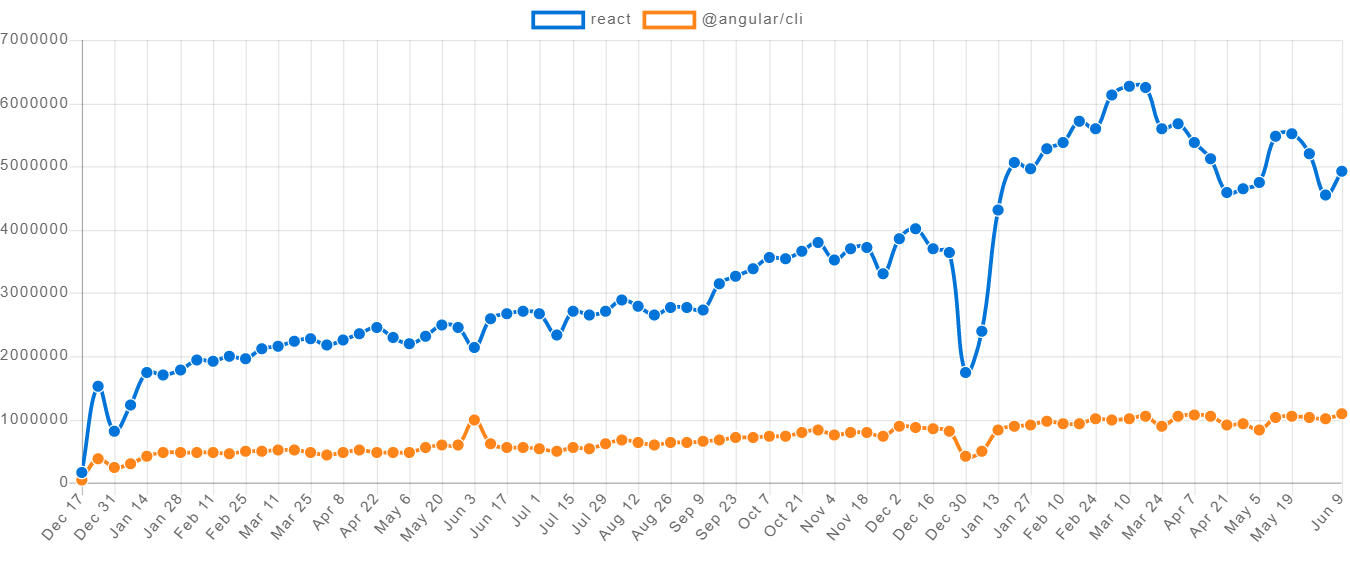
\includegraphics[scale=0.3]{images/npm-trends-react-vs-angular.png}
	\end{center}
	\caption{npm-trends-react-vs-angular}
\end{figure}

\subsection{What are companies using?}

\section{Conclusion}


% 6 pages